\section{Results and discussion}

In this section we detail the findings of our study. We first present the results of each study
in Section~\ref{sec:res-fs} and Section~\ref{sec:res-ss}. In Section~\ref{sec:discussion} we summarize the
implications of our study. 

\subsection{Result of the first study: A non-exact replication}\label{sec:res-fs}

Our first study performed a non-exact replication of Bao et al work.
Our study differs from the original because here we isolated the effect
of the DroidFax static analysis algorithms in the performance to
identify malicious apps using the test case generation tools for
mining sandboxes. In addition, we discarded six pairs of
Android apps we were not able to instrument---out of the $102$ pairs used in the \original work.
\rb{All of this following information should be detailed in
the study settings, and not repeated here if it is already there.} {\color{red}We also introduced a recent test generator tool, that has not been considered at previous work, Humanoid, and different from the original study, we expand the execution time of each test generation tool, executing each app at each tool for three minutes, while the original study executed for just one minute. The purpose of this time expansion is to check if the test generation tool code coverage results are consistent with Bao et al. results.}

As discussed in the previous section, we first executed the analysis using the DroidXP benchmark with its default configuration. After that, we executed the analysis again though disabling the DroidFax static analysis algorithm, so that we could better estimate the performance of the dynamic analysis tools for mining Android sandboxes. Table~\ref{tab:fs} summarizes the results of the execution. The columns Exec. (I) and Exec. (II) 
show the number of malwares identified when executing each tool (I) with the
support of the DroidFax static analysis algorithms and (II) without the support
of DroidFax static analysis algorithms. The Improvement column shows the impact
(in percentage) of DroidFax static analysis algorithms in the results.
In the previous work~\cite{}, the authors do not present a
discussion about the influence of DroidFax in the results, even
though here we report that this difference is in the
range from 23.94\% (Monkey) to 69.39\% (Humanoid)---discarding our
\joke tool for which DroidFax improves its performance in 100\% (as expected).
Next we discuss the result of each individual test generation tool. 

\begin{table}[ht]
  \caption{Summary of the results of the first study. }
  \centering
  \begin{small}
 \begin{tabular}{lrrr}
   \toprule
   Tool & Exec. (I) & Exec. (II) & Improvement (\%) \\   \midrule
  Monkey &  71 &  54 & 23.94 \\ 
  DroidMate &  64 &  48 & 25.00 \\ 
  DroidBot &  68 &  54 & 20.59 \\ 
  Humanoid &  49 &  15 & 69.39 \\ 
  \joke &  42 &   0 & 100.00 \\ 
 \bottomrule
 \end{tabular}
 \end{small}
 \label{tab:fs}
\end{table}


\subsubsection*{Monkey} sandbox for the first execution (Exec. (I)) detected more apps with malicious behavior than any other tool considered in our study (71 out of the 96 pairs of Android apps). Contrasting, in the original study, Monkey got the third-best performance, detecting 48 malwares within the 102 pairs (47.05\%). This difference might be due to the Monkey randomly strategy for test case generation. \rb{I am not convinced that the other tools do not employ any randomness.} For our second execution (Exec. (II)), there is a reduction of 23.94\% in the Monkey's performance, totaling 54 malware detected---which matches the performance of DroidBot for Exec. (II). \rb{Considering only one run for each configuration, that is Exec. (I) and Exec. (II), we cannot assure that the difference is due to disabling the DroidFax static analysis algorithms.}


\subsubsection*{DroidBot} in the first execution (Exec. (I)) its resulting sandbox detected a total of 68 malware among $96$ pairs analyzed (70.83\%). Interesting, this is the same performance of the original study---although the original study analyzed $102$ pairs of Android apps. Also, in the original study, DroidBot was the test case generation tool whose resulting sandbox detected the largest number of malicious apps. However, in our second execution (Exec. (II)), its performance decreased in 20.58 \%. \rb{Not sure if the following sentence is right.} Despite this reduction, it achieved the largest number of malicious apps detected in the second execution.

\subsubsection*{DroidMate} in the first execution led to a sandbox that detected 64 apps with malicious behavior (66.66\%). Contrasting, in the original study DroidMate detected 54 among 102 (52.94\%). A possible explanation for this difference is that here we use the more recent version of DroidMate. In the second execution, without the DroidFax static analysis algorithms, the resulting sandbox's performance drops by 25\%, being able to detect 48 out of the 96 pairs of Android apps. 


\subsubsection*{Humanoid} presented the worse performance, even though a previous
work~\cite{DBLP:conf/kbse/LiY0C19} shows that it presents the highest lines coverage in comparison to Monkey, DroidBot, and DroidMate. In the first execution (Exec. (I)), the resulting Humanoid sandbox identified 49 malwares in our dataset (51.04\%). Since Bao et al. did not explored Humanoid in their study, we do not have a baseline for comparison. Regarding the second execution, without static analysis, Humanoid was the most affected by disabling the DroidFax static analysis algorithm, losing 69.38\% of its effectiveness, and being able to detect just 15 malwares.

\subsubsection*{\joke} is our fake test case generation tool that we use to help us understand the performance of the DroidFax static analysis algorithm for mining sandboxes. We integrated \joke into the DroidXP benchmark as an additional test generation tool that does not run the Android apps during the benchmark execution. As a result, the analysis using \joke reveals the performance of DroidFax static analysis algorithms only. For the first execution, with the DroidFax static algorithms enabled, even though \joke does not execute the Android apps, its resulting sandbox detected 43.75\% of the malwares. For the second execution, that is, disabling the DroidFax static analysis algorithm, the resulting \joke sandbox was unable to detect any malware. This result was expected, since \joke does not analyze the Android apps during the benchmark execution.

\begin{finding}
  Integrating the dynamic analysis tools
  with the DroidFax static analysis algorithms
  improves substantially the performance
  of the resulting Android sandboxes for
  detecting malicious behavior. 
\end{finding}
 
The Venn-diagram of Figure~\ref{fig:venn-plot1}
summarizes how the tools can complement each other.
Note in the diagram that 47 malwares have been detected by all sandboxes generated in the first execution (with the DroidFax static analysis algorithms), out of the 77 identified by at least one sandbox. In addition, the DroidBot sandbox did not detect any malware that had not been detected by the other tools. Differently, the Monkey's sandbox detected five malwares that had not been detected by any other sandbox, DroidBot sandbox detected four malwares that had not been detected by any other sandbox, and Humanoid detected one malware that had not been detected by any other sandbox. Contrasting with the Bao et al. work~\cite{DBLP:conf/wcre/BaoLL18},
our results suggest that using DroidBot in combination with Monkey, DroidMate, and Humanoid does not improve the general performance of an integrated environment for mining
Android sandboxes.  

\begin{finding}
  Our results suggest that one might benefit from using  an integrated
  environment that combines Monkey, DroidMate, and Humanoid to
  mine Android sandboxes. Introducing the DroidBot 
  tool does not improve the results.
\end{finding}


\begin{figure}[htb]
  \centering{
  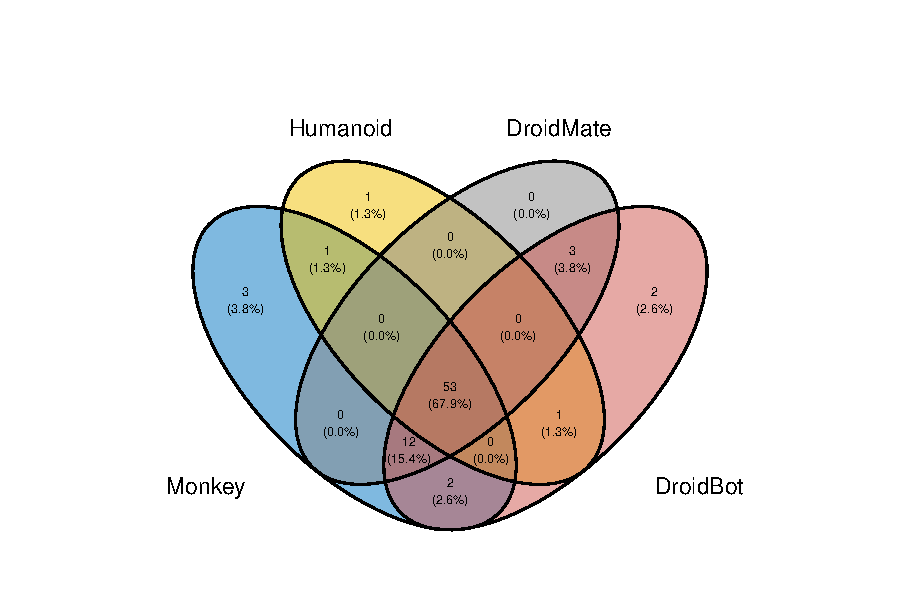
\includegraphics[trim=60 20 0 50,scale=0.7]{images/venn-plot-s1-1.pdf}}
  \caption{Venn Diagram highlighting how the sandboxes from the tools can
    complement each other.}
  \label{fig:venn-plot1}
\end{figure}


Altogether, ignoring the \joke tool, our study reveals that from 51.04\% (Humanoid)
to 73.95\% (Monkey) of the malicious apps investigated in our study can be
detected using the sandboxes generated after running the test case tools with the support of DroidFax static analysis algorithms. Besides that, in the first execution, none of the resulting sandboxes could detect 19 malwares in our dataset (19.79\%). According to the Euphony tool~\cite{hurier2017euphony}, 13 of these 19 malwares are \emph{adwares}, three are \emph{trojans}, two are PUPs (\emph{Potentially Unwanted Program}), and one is an \emph{exploit}. \rb{In what follows we present some characteristics of malwares that had not been detected by the sandboxes.}

\rb{This is an interesting place to present the details of two or three malwares in this set of 19 malwares that had not been detected by any tool. I think Thales could work on this, since he has helped Handrick to dissect the malwares.}



\subsection{Result of the second study: Tainted analysis algorithms.}\label{sec:res-ss}

In this second study we used a tainted analysis approach to mine differences between the benign and malicious versions of each of the 96 Android apps in our dataset. To this end we leverage the FlowDroid tool, which tracks how sensitive information flows through the apps using tainted analysis algorithms. Regarding accuracy, the tainted analysis approach detected 58 out of the 96 pairs in our dataset (60,42\%), that is, the FlowDroid approach leads to a better performance than any sandbox originated in the second execution of the dynamic analysis tools (without the DroidFax static analysis algorithms).

\begin{finding}
  The performance of FlowDroid to identify malicious behavior
  using our approach is superior than the performance of the
  mining sandbox approach supported by dynamic analysis only---without
  the DroidFax static analysis algorithms.
\end{finding}

Additionally, we investigate if we could benefit from combining
the results from FlowDroid and DroidFax. Figure~\ref{fig:venn-plot2} shows a
Venn-diagram summarizing the results. So, when combining
the results from FlowDroid and DroidFax, we were able to detect
67 of the malicious apps (69.79\%), a performance compatible
to that we found as response to the first execution of the
test case generation tools---which also considers the DroidFax
static analysis algorithms. More interesting, from those 67
malicious apps identified, 33 pairs had been found by
both tools (FlowDroid and DroidFax), even though they follow
a completely different static analysis approach. Furthermore,
FlowDroid shows to bem more effective than DroidFax, detecting 25 malicious
apps that had not been detected by DroidFax (while DroidFax detected nine
malicious apps that had not been detected by FlowDroid).

\begin{finding}
  Integrating the results of static analysis tools
  (such as FlowDroid and DroidFax) seems promising,
  leading to a performance similar to that achievend
  when combining test case generation tools with the
  DroidFax tool. 
\end{finding}

\begin{figure}
  \centering{
  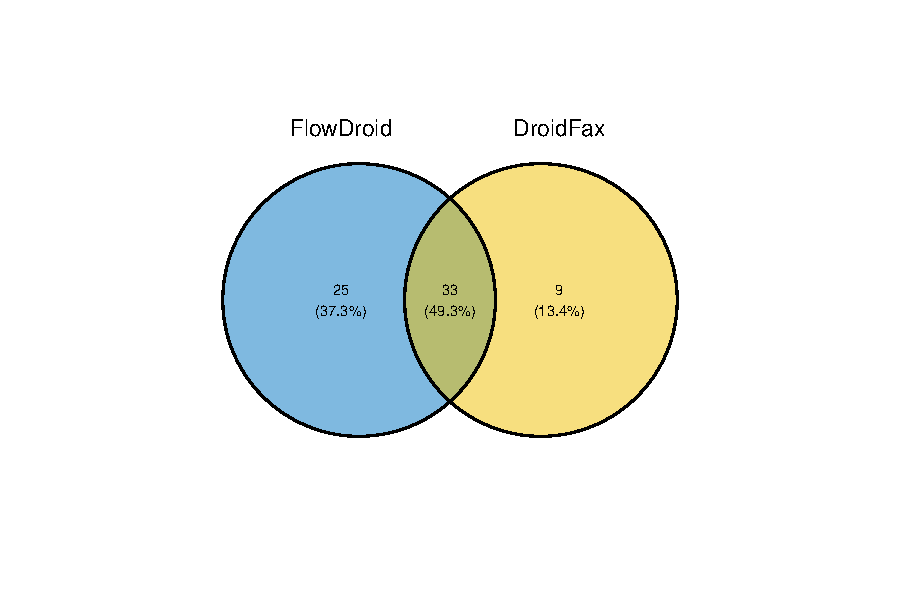
\includegraphics[trim=60 20 0 50,scale=0.7]{images/venn-plot-s2-1.pdf}}
  \caption{Venn Diagram highlighting the possible benefits of
    integrating FlowDroid and DroidFax.}
  \label{fig:venn-plot2}

\end{figure}

The execution of FlowDroid is also feasible: the analysis takes only
32.08 seconds per app on average, totaling a processing time of 52
minutes to analyze all 96 pairs of Android apps.
Even though the time to execute the FlowDroid analysis depends on the size
of the app, the longest run took only 437 seconds. 

Finally, we can highlight that FlowDroid was able to detect four malwares among the 19 malicious Android apps that had not
been detected by the sandboxes constructed in the first study. Among these
four malwares, two are \emph{trojans}, 1 is an \emph{exploit}, and 1
is an \emph{adware}.

\begin{finding}
  Although FlowDroid presents a performance similar
  to that of using the dynamic analysis approach for mining sandboxes,
  it was able to detect only four additional malwares (out of the
  19) that had not been detected in the first study. 
\end{finding}

\rb{This is a nice place to present some details about the malwares
  that FlowDroid had detected, showin the additional source-sink pairs
  that emmerged. A discussion about these aforementioned four pairs would
  also be relevant.}

\rb{I finished my first review until this place. Tomorrow I will continue
from here.} 


\subsection{Discussion}\label{sec:discussion}

First we find that static analysis summaries had impact in the Bao et al. study. It was responsible for improving the results of the tools by 47.78\% than its executions alone, answering our first research question (RQ1). Second, Table \ref{tab:malwareWithout} summarizes our findings addressing the second research question (RQ2). We realized that disregarding the static analysis algorithms, and discarding Joke tool, among the tools analyzed in your study, Humanoid had the biggest performance drop, and the least affected was DroidBot, proving be the tool with better effective performance, in terms of the number of detected malware. Finally, we answered our last research question (RQ3) when we leverage sandboxes, complementing the dynamic analysis provided by test generation tool with tainted analysis algorithms. Our experiment highlight that 69.79\%-81.25\% of malware in dataset can be now uncovered by the complement of tainted analysis algorithms, evidencing that 
sandboxes can be further boosted when coupled with new static analysis techniques. We found that the number of identified malicious apps detected is increased for all cases, achieving at the best case, 81.25\% with Monkey, a better performance than all five tools explored at Bao et al., even when they combined all the tools together at theirs work 75.49\%. Table \ref{tab:tanted} display the increase of all tools explored at our research.

\begin{table}[ht]
\centering
\begin{tabular}{lccc}\toprule
 Test Generation & FlowDroid & Total & \%\\
 Tool & Increase  &  & \\ \midrule
 Monkey & 7 & 78 & 81.25\\
 DroidMate & 10 &  74 & 77.08 \\
 Humanoid & 20 & 69 & 71.87  \\
 Joke & 25 & 67 & 69.79 \\
 DroidBot & 9 & 77 & 80.20  \\\midrule
 
\end{tabular} 
\caption{Malwares detected in 96 pair (B/M) increased by Tainted analysis Algorithms}
\label{tab:tanted}
\end{table}

%%here we also have to write about the intersection between droidfax and tainted analysis now, and about what 1 reveled and other dont, and otherwise. 


%Here we can write about MOTIVATION EXAMPLES.
